\begin{frame}
    \frametitle{\problemtitle}
    \begin{itemize}
        \item<+-> \textbf{Problème:} Étant donné une distance $d$ et un angle $\alpha$ dans un triangle rectangle, trouver le double de la longueur du côté opposé à l'angle.
        \begin{figure}
            \centering
            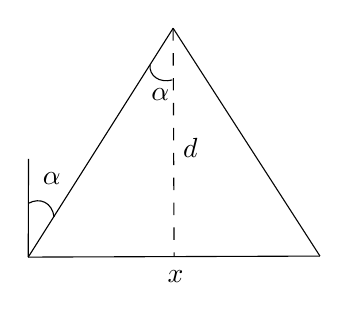
\begin{tikzpicture}[x=0.75pt,y=0.75pt,yscale=-1,xscale=1]
                %Straight Lines [id:da37855877491674694]
                \draw [color={rgb, 255:red, 0; green, 0; blue, 0 }  ,draw opacity=0.98 ]   (289.42,49.79) -- (360.17,159.57) ;
                %Curve Lines [id:da24698423041058837]
                \draw    (278.27,67.51) .. controls (277.87,72.71) and (282.67,76.31) .. (289.07,74.71) ;
                %Straight Lines [id:da4048989193409195]
                \draw    (289.42,49.79) -- (219.61,160.06) ;
                %Straight Lines [id:da7530300672363276]
                \draw  [dash pattern={on 4.5pt off 4.5pt}]  (289.42,49.79) -- (289.89,159.82) ;
                %Straight Lines [id:da9159813820949739]
                \draw    (219.61,160.06) -- (360.17,159.57) ;
                %Curve Lines [id:da2898873933117663]
                \draw    (219.75,134.12) .. controls (225.42,131.12) and (231.08,133.79) .. (232.07,140.71) ;
                %Straight Lines [id:da10125468748115951]
                \draw    (219.75,112.79) -- (219.61,160.06) ;

                % Text Node
                \draw (277.71,77.84) node [anchor=north west][inner sep=0.75pt]   [align=left] {$\displaystyle \alpha $};
                % Text Node
                \draw (292.99,101.47) node [anchor=north west][inner sep=0.75pt]   [align=left] {$\displaystyle d$};
                % Text Node
                \draw (285.47,165.2) node [anchor=north west][inner sep=0.75pt]   [align=left] {$\displaystyle x$};
                % Text Node
                \draw (225.37,117.84) node [anchor=north west][inner sep=0.75pt]   [align=left] {$\displaystyle \alpha $};
            \end{tikzpicture}
       \end{figure}
        \item<+-> Simple trigonométrie : $x=2d\cdot\tan(\alpha)$ (n'oubliez pas de passer $\alpha$ en radians).
    \end{itemize}
    % \solvestats
\end{frame}
